\documentclass[11pt,a4paper]{report}
\usepackage[T1]{fontenc}
\usepackage{mathpazo}
\usepackage[scaled=.92]{helvet}
\usepackage{courier}
\usepackage[a4paper,margin=2.4cm]{geometry}
\usepackage{microtype,xcolor,graphicx,booktabs,array,enumitem,amsmath,amssymb}
\usepackage{tikz}
\usetikzlibrary{positioning,arrows.meta,shapes.geometric,fit,calc,backgrounds}
\usepackage[most]{tcolorbox}
\usepackage{listings}
\usepackage{fancyhdr}
\usepackage{titlesec}
\usepackage{caption}
\usepackage[colorlinks=true,linkcolor=ink,urlcolor=teal,citecolor=ink]{hyperref}

% ---------- editable metadata ----------
\newcommand{\authorname}{Tulja}
\newcommand{\repourl}{https://github.com/<tuljayerram>/netra-ai}

% ---------- colours ----------
\definecolor{ink}{HTML}{0B3C5D}
\definecolor{teal}{HTML}{1B7F79}
\definecolor{saffron}{HTML}{D9822B}
\definecolor{paper}{HTML}{F5F7F9}
\definecolor{codegray}{HTML}{6B7785}

% ---------- helpers ----------
\usepackage{url}
\urlstyle{tt}
\def\UrlBreaks{\do\/\do\_\do\.\do\-\do\=\do\(\do\)\do\,\do\:}
\DeclareRobustCommand{\code}[1]{\path{#1}}
\setlist{itemsep=2pt,topsep=4pt}
\setlength{\parskip}{4pt}
\setlength{\parindent}{0pt}
\captionsetup{font=small,labelfont={bf,color=ink}}

\titleformat{\chapter}[hang]{\normalfont\huge\bfseries\color{ink}}{\thechapter}{16pt}{}[\vspace{2pt}\color{saffron}\titlerule]
\titleformat{\section}{\normalfont\Large\bfseries\color{ink}}{\thesection}{10pt}{}
\titleformat{\subsection}{\normalfont\large\bfseries\color{teal}}{\thesubsection}{8pt}{}
\titlespacing*{\chapter}{0pt}{-10pt}{18pt}

\pagestyle{fancy}
\fancyhf{}
\fancyhead[L]{\small\color{codegray}NetraAI tutorial}
\fancyhead[R]{\small\color{codegray}\leftmark}
\fancyfoot[C]{\small\thepage}
\renewcommand{\headrulewidth}{0.3pt}

% ---------- boxes ----------
\newtcolorbox{notebox}[1][Note]{enhanced,breakable,colback=teal!6,colframe=teal,
  fonttitle=\bfseries,title={#1},boxrule=0.6pt,arc=2pt,left=6pt,right=6pt}
\newtcolorbox{warnbox}[1][Caution]{enhanced,breakable,colback=saffron!10,colframe=saffron,
  fonttitle=\bfseries,title={#1},boxrule=0.6pt,arc=2pt,left=6pt,right=6pt}
\newtcolorbox{safetybox}[1][Safety statement]{enhanced,breakable,colback=red!5,colframe=red!60!black,
  fonttitle=\bfseries,title={#1},boxrule=0.8pt,arc=2pt,left=6pt,right=6pt}

% ---------- listings ----------
\lstdefinestyle{base}{basicstyle=\ttfamily\footnotesize,breaklines=true,breakatwhitespace=false,
  columns=fullflexible,keepspaces=true,showstringspaces=false,frame=single,rulecolor=\color{ink!35},
  backgroundcolor=\color{paper},xleftmargin=2pt,xrightmargin=2pt,aboveskip=8pt,belowskip=6pt,
  keywordstyle=\bfseries\color{ink},commentstyle=\itshape\color{codegray},stringstyle=\color{teal},
  captionpos=b,literate={~}{{\textasciitilde}}1}
\lstdefinestyle{py}{style=base,language=Python,numbers=left,numberstyle=\tiny\color{codegray},numbersep=6pt}
\lstdefinestyle{sh}{style=base,language=bash,morekeywords={sudo,apt,git,pip,python,ollama,curl,source,mkdir,cd,touch,wsl,usbipd,streamlit,pytest}}
\lstdefinestyle{plain}{style=base}

\emergencystretch=4em
\begin{document}

% ================= TITLE PAGE =================
\begin{titlepage}
\begin{tikzpicture}[remember picture,overlay]
  \fill[ink] (current page.north west) rectangle ([yshift=-9.2cm]current page.north east);
  \fill[saffron] ([yshift=-9.2cm]current page.north west) rectangle ([yshift=-9.45cm]current page.north east);
  % stylised eye
  \begin{scope}[shift={([xshift=-4cm,yshift=-4.6cm]current page.north east)}]
    \draw[white,line width=1.6pt] (-1.5,0) .. controls (-0.7,1.0) and (0.7,1.0) .. (1.5,0)
                                   .. controls (0.7,-1.0) and (-0.7,-1.0) .. (-1.5,0);
    \fill[saffron] (0,0) circle (0.42);
    \fill[white] (0.12,0.12) circle (0.1);
  \end{scope}
\end{tikzpicture}
\vspace*{1.2cm}
{\color{white}\Huge\bfseries NetraAI\par}
\vspace{6pt}
{\color{white}\Large An Intelligent Image and Video Processing Agent\\ for Assistive Vision\par}
\vspace{2.4cm}
{\Large\bfseries\color{ink} A detailed, command-by-command tutorial\\ using free and open-source tools on Ubuntu (WSL2)\par}
\vspace{1cm}
{\large Local LLM tool calling $\cdot$ OpenCV $\cdot$ YOLO $\cdot$ OCR $\cdot$ speech $\cdot$ edge deployment\par}
\vfill
{\large\authorname\par}
{\normalsize Technical tutorial \quad $\cdot$ \quad November 2026\par}
{\small Companion code: \url{\repourl}\par}
\end{titlepage}

\begin{abstract}
\noindent This tutorial shows how to design, install, program, test and publish a locally running AI agent
for image and video processing in an \emph{assistive-vision} setting: a camera worn by, or carried with, a
person with visual impairment, and software that turns frames into short spoken information.
A local large language model (LLM) served by Ollama interprets natural-language instructions and selects tools
from a fixed allow-list. Established libraries perform the numerical work: OpenCV and scikit-image for enhancement,
filtering and metrics; a small YOLO detector for objects; Tesseract for printed text; espeak-ng for speech.
The tutorial covers WSL2/Ubuntu setup, the tool library, a bounded agent loop, a left/center/right and proximity
guidance layer, controlled experiments, evaluation metrics, a Streamlit interface, edge-deployment considerations for
a Raspberry Pi-class device, safety and privacy practice, and step-by-step publication to GitHub. All code
is in the companion repository and is included in this document by reference, so the text and the code cannot drift apart.
\end{abstract}

\tableofcontents

% =====================================================================
\chapter{Introduction}
% =====================================================================

\section{What is an assistive-vision agent?}
An \emph{image and video processing (IVP) agent} accepts a request in natural language, decides which
computer-vision operation fits, runs it, checks the result and reports what it did. For an assistive-vision project the
camera is the sensor and the user is a person who cannot rely on sight alone. Typical needs are:
knowing what is in front of them and roughly where, reading printed labels, and getting information in a form they can
use immediately, which usually means speech rather than a picture.

The language model is the \emph{coordinator}, not the vision engine. It never touches pixels. It reads the request,
picks a function such as \code{enhance_low_light} or \code{detect_objects}, and explains the result. OpenCV,
scikit-image, YOLO, Tesseract and espeak-ng do the actual computation, and their outputs are deterministic and measurable.

\section{Why this domain}
Assistive vision is a good teaching domain because it forces engineering trade-offs that generic image-processing
exercises hide.
\begin{itemize}
  \item \textbf{Latency matters.} A description that arrives three seconds late may describe a scene the user has already left.
  \item \textbf{Bad input is normal.} A camera on a moving head sees motion blur, low light, glare and awkward angles. Image-quality assessment and enhancement are part of the pipeline, not an optional extra.
  \item \textbf{Errors have asymmetric cost.} Missing a hazard is worse than a false alarm, but too many false alarms make a user stop listening. This is why evaluation here goes beyond accuracy.
  \item \textbf{Edge constraints are real.} The final device is typically a small single-board computer with limited memory, so model size, input resolution and frame rate become design variables.
  \item \textbf{Privacy is not optional.} A wearable camera records bystanders. Local processing keeps frames on the device.
\end{itemize}

\begin{safetybox}
NetraAI is a research and teaching prototype. It is \textbf{not} a certified mobility or safety device. It must not
replace a white cane, a guide dog or orientation-and-mobility training. Detections are estimates; the system never
announces that a path is ``clear'', only which known objects it detected. Any evaluation with visually impaired
participants needs ethical approval, informed consent and involvement of qualified mobility instructors.
\end{safetybox}

\section{Example requests}
The finished agent should handle requests such as:
\begin{itemize}
  \item ``Is \code{hallway.png} too dark? If so, enhance it and tell me what you changed.''
  \item ``Detect objects in \code{street.png} and tell me where the closest one is.''
  \item ``Read the text on \code{medicine_box.png} in English and Telugu.''
  \item ``Extract one frame every two seconds from \code{walk.mp4}.''
  \item ``Darken \code{astronaut.png}, enhance it, and compare PSNR and SSIM against the original.''
  \item ``Analyse \code{crossing.mp4} every half second and save a guidance timeline.''
  \item ``Run the full navigation pipeline on \code{corridor.png} and give me the audio file.''
\end{itemize}

\section{Architecture}
Figure~\ref{fig:arch} separates five responsibilities: interaction, reasoning, controlled tool execution, deterministic
vision processing, and presentation. The controller is the trust boundary. The model proposes; the controller validates and executes.

\begin{figure}[ht]
\centering
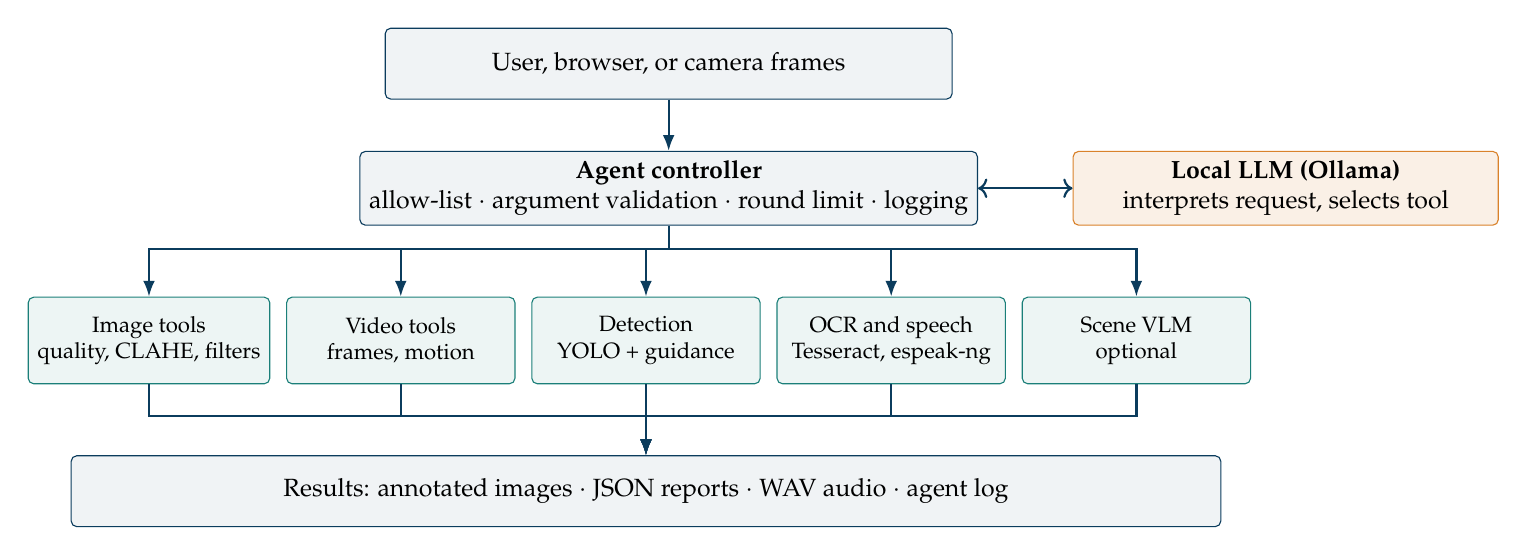
\begin{tikzpicture}[node distance=6.5mm,
  box/.style={draw=ink,rounded corners=2pt,fill=ink!6,align=center,font=\small,minimum height=9mm},
  tool/.style={draw=teal,rounded corners=2pt,fill=teal!8,align=center,font=\footnotesize,minimum height=11mm,minimum width=2.9cm},
  arr/.style={-{Latex[length=2mm]},thick,ink}]
\node[box,minimum width=7.2cm] (user) {User, browser, or camera frames};
\node[box,minimum width=7.2cm,below=of user] (ctrl) {\textbf{Agent controller}\\ allow-list $\cdot$ argument validation $\cdot$ round limit $\cdot$ logging};
\node[box,minimum width=5.4cm,right=12mm of ctrl,fill=saffron!12,draw=saffron] (llm) {\textbf{Local LLM (Ollama)}\\ interprets request, selects tool};
\node[tool,below=9mm of ctrl,xshift=-6.6cm] (t1) {Image tools\\ quality, CLAHE, filters};
\node[tool,right=2mm of t1] (t2) {Video tools\\ frames, motion};
\node[tool,right=2mm of t2] (t3) {Detection\\ YOLO + guidance};
\node[tool,right=2mm of t3] (t4) {OCR and speech\\ Tesseract, espeak-ng};
\node[tool,right=2mm of t4] (t5) {Scene VLM\\ optional};
\node[box,minimum width=14.6cm,below=9mm of t3] (res) {Results: annotated images $\cdot$ JSON reports $\cdot$ WAV audio $\cdot$ agent log};
\draw[arr] (user) -- (ctrl);
\draw[arr,<->] (ctrl) -- (llm);
\draw[arr] (ctrl.south) -- ++(0,-3mm) -| (t3.north);
\foreach \t in {t1,t2,t4,t5} {\draw[arr] (ctrl.south) ++(0,-3mm) -| (\t.north);}
\foreach \t in {t1,t2,t3,t4,t5} {\draw[arr] (\t.south) -- ++(0,-4mm) -| (res.north);}
\end{tikzpicture}
\caption{Logical architecture of NetraAI. Only functions in the allow-list can be executed.}
\label{fig:arch}
\end{figure}

\section{Why a local, open-source stack?}
A local system keeps camera frames on the user's computer, avoids recurring service cost, works offline after the
initial downloads, and is reproducible because algorithms, parameters and versions can be recorded.
``Free and open source'' needs a qualification: a library may be open source while a particular \emph{model weight},
dataset, or commercial deployment has additional conditions. This matters here because the detector used in this tutorial
is distributed under a licence with obligations for distribution and network use (Chapter~\ref{ch:detect}).
Always read the licence of the exact version you ship.

\section{What you will build}
The companion repository has the following layout. Every listing in this document is included directly from these files.
\begin{lstlisting}[style=plain]
netra-ai/
|-- netra/
|   |-- common.py        safe paths, limits, image I/O
|   |-- image_tools.py   quality, enhancement, filters, edges, segmentation
|   |-- video_tools.py   metadata, frame sampling, motion detection
|   |-- spatial.py       zones, proximity, guidance sentence, throttle
|   |-- detection.py     YOLO inference, annotated output, video timeline
|   |-- ocr_tools.py     Tesseract text reading
|   |-- speech.py        espeak-ng text-to-speech to WAV
|   |-- vision_tools.py  vision-language scene description
|   |-- metrics.py       PSNR, SSIM, IoU, precision/recall, low-light simulator
|   |-- pipeline.py      assess -> enhance -> detect -> speak
|   |-- agent.py         allow-listed tool-calling loop
|   `-- live.py          webcam / video-file guidance loop
|-- app.py               Streamlit interface
|-- tests/               pytest suite
|-- scripts/             setup_ubuntu.sh, run_lowlight_experiment.py
|-- docs/                this tutorial (LaTeX source and PDF)
`-- README.md, LICENSE, requirements*.txt, .gitignore, .github/workflows/ci.yml
\end{lstlisting}

\begin{notebox}[Validation status of the companion code]
The image tools, video tools, spatial guidance, metrics, tool schemas, allow-list behaviour and the detection
post-processing (with a stand-in model) are covered by an automated test suite that passes (20 tests). The low-light
experiment in Chapter~\ref{ch:experiments} was actually run and its numbers are reported as measured.
\textbf{Not exercised when this tutorial was prepared:} real YOLO inference, tool calling against a live Ollama model,
Tesseract and espeak-ng output, webcam capture, and Raspberry Pi deployment. Treat those parts as a checklist to verify on
your own machine and record your results (Chapter~\ref{ch:eval}).
\end{notebox}

% =====================================================================
\chapter{Software Stack and Responsibilities}
% =====================================================================
\begin{table}[ht]
\centering\small
\begin{tabular}{@{}p{3.1cm}p{3.6cm}p{8.2cm}@{}}
\toprule
\textbf{Component} & \textbf{Software} & \textbf{Purpose}\\
\midrule
Operating system & Ubuntu 24.04 LTS (native or WSL2) & Development and execution platform.\\
Language & Python 3 & Tool functions, agent controller, tests.\\
Model runtime & Ollama & Runs LLMs locally and exposes an HTTP API with tool calling.\\
Language model & Llama or Qwen family & Interprets requests and chooses tools.\\
Computer vision & OpenCV (headless build) & I/O, colour conversion, CLAHE, filters, edges, contours, background subtraction.\\
Analysis & NumPy, scikit-image & Array maths, PSNR and SSIM.\\
Plots & Matplotlib & Histograms and experiment figures.\\
Detection & Ultralytics YOLO (nano model) & Object classes and bounding boxes.\\
Text reading & Tesseract OCR & Printed text, including Indian-language packs.\\
Speech & espeak-ng & Offline text-to-speech to WAV.\\
Video & FFmpeg & Decoding, encoding, standard conversions.\\
Interface & Streamlit & Local browser interface.\\
Quality & pytest, GitHub Actions & Regression tests and continuous integration.\\
Publishing & Git, GitHub & Version control and sharing.\\
\bottomrule
\end{tabular}
\caption{Components and their roles.}
\end{table}

\paragraph{OpenCV.} The workhorse for conventional computer vision. This tutorial uses \code{imread}, \code{imwrite},
\code{cvtColor}, \code{createCLAHE}, \code{LUT}, \code{medianBlur}, \code{GaussianBlur}, \code{bilateralFilter},
\code{Canny}, \code{threshold}, \code{Laplacian}, \code{VideoCapture}, \code{VideoWriter} and
\code{createBackgroundSubtractorMOG2}. The \emph{headless} wheel (\code{opencv-python-headless}) is used because it has no GUI dependencies,
which avoids the shared-library errors that the standard wheel can produce on servers and in WSL.

\paragraph{FFmpeg.} Better than OpenCV for standard media transformations (resize, trim, re-encode) and for timestamp-accurate work.
OpenCV is convenient when you need custom frame-by-frame algorithms.

\paragraph{Ollama.} Provides a local model runtime and an HTTP API. The agent sends a prompt and a list of tools; the model may answer with a
tool call; the Python controller validates and executes it, then returns the result to the model.

\paragraph{YOLO, Tesseract, espeak-ng.} These are the three assistive components: \emph{what} is in the frame, \emph{what the text says}, and \emph{how to say it aloud}.

% =====================================================================
\chapter{Ubuntu Development Environment}
% =====================================================================
This chapter targets Ubuntu 24.04 LTS, either installed natively or running under Windows through WSL2. Ubuntu-specific steps are the same in both.

\section{Windows users: install WSL2 with Ubuntu}
In an administrator PowerShell window:
\begin{lstlisting}[style=sh]
wsl --install -d Ubuntu-24.04
\end{lstlisting}
\begin{itemize}
  \item \code{wsl --install} enables the WSL features and installs a Linux distribution; \code{-d} selects the distribution.
  \item Restart if asked, then create a Linux username and password in the Ubuntu window that opens.
\end{itemize}
Verify and update:
\begin{lstlisting}[style=sh]
wsl -l -v
wsl --update
\end{lstlisting}
\code{-l -v} lists installed distributions with their WSL version; the Ubuntu entry should show version 2.

\begin{notebox}[WSL practicalities]
\begin{itemize}
  \item \textbf{Work inside the Linux filesystem} (\code{~/}), not under \code{/mnt/c/}. File access across the boundary is much slower, which hurts video processing.
  \item \textbf{systemd.} Ollama's installer sets up a service. On recent WSL, Ubuntu enables systemd by default; if \code{systemctl status} reports that it is not running, add \code{[boot]} and \code{systemd=true} to \code{/etc/wsl.conf}, then run \code{wsl --shutdown} from PowerShell and reopen Ubuntu.
  \item \textbf{GPU.} Install the NVIDIA driver on Windows (not inside Ubuntu); CUDA-enabled tools in WSL use it. Check with \code{nvidia-smi} inside Ubuntu. CPU is enough for this tutorial.
  \item \textbf{Audio.} WSLg normally provides audio. Play a generated WAV with \code{paplay file.wav} after installing \code{pulseaudio-utils}.
  \item \textbf{Webcam.} A USB camera can be forwarded with \code{usbipd-win}, but the default WSL kernel may lack camera (UVC) drivers. The simplest route is to develop with recorded video files in WSL and run the live camera loop on native Ubuntu or the Raspberry Pi. Check Microsoft's current WSL documentation before investing time here.
\end{itemize}
\end{notebox}

\section{Update package information}
\begin{lstlisting}[style=sh]
sudo apt update
sudo apt upgrade -y
\end{lstlisting}
\code{sudo} runs a command as administrator; \code{apt} is Ubuntu's package manager; \code{update} refreshes the package index; \code{upgrade} installs newer versions of installed packages; \code{-y} answers yes to prompts (review changes first on a production machine).

\section{Install system dependencies}
\begin{lstlisting}[style=sh]
sudo apt install -y python3 python3-pip python3-venv python3-dev \
    build-essential git curl wget ffmpeg \
    tesseract-ocr tesseract-ocr-tel tesseract-ocr-hin espeak-ng
\end{lstlisting}
The trailing backslash continues the command on the next line.
\begin{description}[leftmargin=3.2cm,style=nextline,font=\ttfamily\small]
  \item[python3, -pip, -venv, -dev] Interpreter, package installer, virtual environments, and headers for compiled extensions.
  \item[build-essential] Compiler and build tools used by some Python packages.
  \item[git, curl, wget] Version control and download tools (curl is also used by the Ollama installer).
  \item[ffmpeg] Multimedia decoding and encoding.
  \item[tesseract-ocr] The OCR engine; \code{-tel} and \code{-hin} add Telugu and Hindi language data, which are useful for signs and labels in India.
  \item[espeak-ng] Offline speech synthesis with many languages and voices.
\end{description}
The same list is automated in \code{scripts/setup_ubuntu.sh}.

\section{Verify the installations}
\begin{lstlisting}[style=sh]
python3 --version
ffmpeg -version
git --version
tesseract --list-langs
espeak-ng --version
\end{lstlisting}
Each prints a version or list. Recording versions is part of reproducible research.

\section{Get the project}
Either clone the finished repository, or create the structure yourself.
\begin{lstlisting}[style=sh]
git clone https://github.com/<your-user>/netra-ai.git
cd netra-ai
mkdir -p input/images input/videos output models
\end{lstlisting}
\code{mkdir -p} creates directories and any missing parents without error if they exist. \code{input/} holds source media, \code{output/} holds everything generated; keeping them separate preserves originals and makes the workflow auditable.

\section{Create and activate a virtual environment}
\begin{lstlisting}[style=sh]
python3 -m venv .venv
source .venv/bin/activate
python -m pip install --upgrade pip setuptools wheel
\end{lstlisting}
\code{-m venv} runs Python's environment module and creates the isolated \code{.venv} directory. \code{source} runs the activation script in the current shell so that \code{python} and \code{pip} refer to the environment; the prompt gains a \code{(.venv)} prefix. \code{python -m pip} guarantees that pip belongs to the active interpreter. Leave the environment with \code{deactivate}.

\section{Install Python libraries}
\begin{lstlisting}[style=plain,caption={requirements.txt}]
numpy
opencv-python-headless
scikit-image
matplotlib
pillow
pandas
pytesseract
ollama
streamlit
pytest
\end{lstlisting}
\begin{lstlisting}[style=sh]
pip install -r requirements.txt
\end{lstlisting}
\code{-r} reads package names from a file. After the first successful install, record exact versions with \code{pip freeze > requirements.lock.txt} for reproducibility.

\begin{warnbox}
Install \emph{only one} OpenCV wheel variant (\code{opencv-python}, \code{opencv-python-headless} or \code{opencv-contrib-python}) in an environment. Mixing them causes confusing import errors.
\end{warnbox}

\section{Run the test suite}
\begin{lstlisting}[style=sh]
python -m pytest -q
\end{lstlisting}
\code{-q} gives compact output. All tests should pass before you continue. They use a temporary project directory (set through the \code{NETRA_HOME} environment variable in \code{tests/conftest.py}), so they never touch your real images.

% =====================================================================
\chapter{Installing and Configuring Ollama}
% =====================================================================
\section{Install Ollama}
\begin{lstlisting}[style=sh]
curl -fsSL https://ollama.com/install.sh | sh
\end{lstlisting}
\begin{itemize}
  \item \code{-f} fail on HTTP errors; \code{-s} silence the progress meter; \code{-S} still show errors; \code{-L} follow redirects.
  \item The pipe \code{|} sends the downloaded script to \code{sh}, which executes it.
\end{itemize}
This runs a remote script. On a managed or security-sensitive computer, download it first, read it, and follow the official installation documentation. Verify with \code{ollama --version}.

\section{Check the service}
\begin{lstlisting}[style=sh]
systemctl status ollama
sudo systemctl start ollama
sudo systemctl enable ollama
\end{lstlisting}
\code{status} shows whether the service is active; \code{start} starts it now; \code{enable} starts it at boot. The API listens on port 11434. Do not expose this port to an untrusted network.

\section{Download a language model}
\begin{lstlisting}[style=sh]
ollama pull llama3.1:8b
\end{lstlisting}
\code{pull} downloads the named model; \code{8b} is the approximate parameter count. Memory needs depend on quantisation and context length. Pick one model first. An alternative is \code{qwen3:8b}. Check the model's licence and tool-calling capability before institutional or commercial use. To use another model without editing code, set an environment variable:
\begin{lstlisting}[style=sh]
export NETRA_LLM="qwen3:8b"
\end{lstlisting}

\section{Test the model and the API}
\begin{lstlisting}[style=sh]
ollama run llama3.1:8b
curl http://localhost:11434/api/tags
\end{lstlisting}
\code{run} opens an interactive session (leave with \code{/bye}); the \code{/api/tags} endpoint returns the locally available models as JSON. A minimal Python check:
\begin{lstlisting}[style=py]
from ollama import chat
reply = chat(model="llama3.1:8b",
             messages=[{"role": "user", "content": "Explain CLAHE in two sentences."}])
print(reply.message.content)
\end{lstlisting}
The model name must match one that is installed locally.

% =====================================================================
\chapter{Image-Processing Tools}
% =====================================================================
Every tool is a plain Python function that validates its input, performs one operation, saves a \emph{new} file and returns a small dictionary. Small, single-purpose functions are easy for a language model to choose between and easy for you to test.

\section{Shared helpers: safe paths and limits}
\lstinputlisting[style=py,caption={\texttt{netra/common.py}},label=lst:common]{../netra/common.py}
\begin{itemize}
  \item \code{BASE} is the project root, overridable with \code{NETRA_HOME}. Tests use that override.
  \item \code{safe_path} rejects anything that is not a plain filename. A model could emit \code{../../etc/passwd}; \code{Path(filename).name != filename} stops path traversal. It also restricts extensions and checks existence.
  \item \code{load_image} decodes with OpenCV (colour images arrive in \textbf{BGR} order, not RGB), refuses oversized images, and fails loudly on undecodable files rather than returning \code{None}.
  \item \code{save_image} checks the Boolean returned by \code{imwrite}; an agent must not report success for a failed save.
  \item \code{rel} returns project-relative paths so results stay readable and do not leak absolute locations.
\end{itemize}

\section{Image quality assessment}
Before enhancing anything, measure. For an 8-bit grayscale image $I$ of $N$ pixels, the tool computes the mean $\mu$, standard deviation $\sigma$, the entropy of the normalised histogram $p(k)$, and a sharpness score:
\[
H = -\sum_{k=0}^{255} p(k)\log_2 p(k), \qquad
S = \operatorname{Var}\!\big(\nabla^2 I\big),
\]
where $\nabla^2$ is the Laplacian. A sharp image has strong second derivatives at edges, so $S$ is large; a blurred image has small $S$. The brightness rule flags \code{low_light} when $\mu<80$ and \code{overexposed} when $\mu>180$; \code{low_contrast} when $\sigma<35$; \code{possibly_blurry} when $S<100$.

\begin{warnbox}[Heuristics, not truths]
These thresholds are starting points. $S$ depends on image resolution and scene content (a plain wall is ``blurry'' by this measure). Tune all four on frames from your own camera, and keep the \code{note} field in the tool result so the model does not overstate certainty.
\end{warnbox}

\section{Enhancement: CLAHE on lightness, then gamma}
Global histogram equalization maps intensities through the cumulative distribution:
\[
s_k = (L-1)\sum_{j=0}^{k} p_r(r_j), \qquad L=256.
\]
It is simple but can over-amplify noise and wash out scenes with both dark and bright regions. \emph{Contrast Limited Adaptive Histogram Equalization} (CLAHE) works on small tiles and clips each tile's histogram at a limit, which restrains noise amplification.

Applying CLAHE to B, G and R separately shifts colours. The tool instead converts to the CIE \textbf{LAB} space, applies CLAHE to the lightness channel $L$ only, and leaves the colour channels $a,b$ untouched. A \emph{gamma} correction then brightens or darkens through a lookup table:
\[
L_{\text{out}} = 255\left(\frac{L_{\text{in}}}{255}\right)^{1/\gamma}.
\]
With $\gamma>1$ the image brightens; with $\gamma<1$ it darkens. The agent should report \code{clip_limit}, \code{tile_grid} and \code{gamma} so an experiment can be reproduced.

\section{Filtering, sharpening, edges and segmentation}
\begin{itemize}
  \item \textbf{Median} filter replaces each pixel by the median of its neighbourhood, $g(x,y)=\operatorname{median}\{f(s,t):(s,t)\in S_{xy}\}$. It suppresses isolated extreme values (salt-and-pepper noise) and preserves edges better than a linear blur.
  \item \textbf{Gaussian} filter convolves with $G(x,y)=\frac{1}{2\pi\sigma^2}\exp\!\left(-\frac{x^2+y^2}{2\sigma^2}\right)$. It suits roughly Gaussian sensor noise but blurs edges. Kernel sizes must be odd so that the kernel has a centre pixel.
  \item \textbf{Bilateral} filter weights neighbours by spatial \emph{and} intensity distance, smoothing flat regions while keeping edges.
  \item \textbf{Unsharp mask} sharpens with $I_{\text{out}}=(1+a)I-a\,G_\sigma{*}I$, where $a$ is the amount.
  \item \textbf{Canny} edges: smoothing, gradient estimation, non-maximum suppression, double thresholding and hysteresis.
  \item \textbf{Otsu} thresholding chooses the global threshold that maximises between-class variance, so no manual value is needed; uneven illumination still defeats global thresholds.
\end{itemize}

\lstinputlisting[style=py,caption={\texttt{netra/image\_tools.py}},label=lst:imagetools]{../netra/image_tools.py}

\paragraph{Reading the code.}
\begin{itemize}
  \item Each public function has a one-line summary and an \code{Args:} block. The Ollama Python client converts type annotations and these docstrings into the tool description sent to the model, so the docstring is part of the interface, not decoration.
  \item Argument ranges are checked \emph{inside} the tool. Never rely on the model to respect ranges.
  \item \code{matplotlib.use("Agg")} selects a non-interactive backend so plotting works without a display (WSL, servers, CI). \code{plt.close(fig)} releases memory in long-running agents.
  \item Output names are prefixed (\code{enhanced_}, \code{median_}, \dots) so originals are never overwritten.
\end{itemize}

\section{Further OpenCV operations}
\begin{table}[ht]\centering\small
\begin{tabular}{@{}lll@{}}\toprule
\textbf{Operation} & \textbf{Function} & \textbf{Use}\\\midrule
Sobel / Laplacian & \code{cv2.Sobel}, \code{cv2.Laplacian} & Gradient and second-derivative edge maps.\\
Erosion / dilation & \code{cv2.erode}, \code{cv2.dilate} & Shrink or grow foreground regions.\\
Opening / closing & \code{cv2.morphologyEx} & Remove specks or fill small gaps.\\
Contours & \code{cv2.findContours} & Boundaries of binary regions.\\
Hough transform & \code{cv2.HoughLines}, \code{cv2.HoughCircles} & Lines (kerbs, crossings) and circles.\\
Watershed & \code{cv2.watershed} & Separate touching objects from markers.\\
\bottomrule\end{tabular}
\end{table}

% =====================================================================
\chapter{Video-Processing Tools}
% =====================================================================
\section{Properties, sampling and motion}
For $N_f$ frames at $f$ frames per second the nominal duration is $T=N_f/f$. This depends on container metadata and is unreliable for variable-frame-rate video; use FFmpeg or timestamp-aware decoding when precision matters.

To sample one frame every $\Delta t$ seconds, the code keeps every $\lceil f\,\Delta t\rfloor$-th frame (\code{round(fps * interval)}).

Motion detection uses \emph{MOG2} background subtraction, which models each pixel as a mixture of Gaussians and flags pixels that do not fit the learned background. Its mask labels shadows with the value 127, so the code thresholds at 200 to discard them, applies a morphological opening to remove specks, and keeps only regions larger than \code{min_area_fraction} of the frame.

\begin{warnbox}[Camera motion]
Background subtraction assumes a \emph{still} camera. On a head-mounted or walking camera the whole scene moves, so almost every pixel is flagged. Use motion detection here as a baseline for static-camera clips (for example a fixed camera at a crossing), and use the object detector for wearable footage.
\end{warnbox}

\lstinputlisting[style=py,caption={\texttt{netra/video\_tools.py}},label=lst:video]{../netra/video_tools.py}

\section{FFmpeg from the terminal}
\begin{lstlisting}[style=sh]
ffmpeg -i walk.mp4 -vf fps=1 frame_%04d.jpg          # one frame per second
ffmpeg -i walk.mp4 -vf scale=640:-2 walk_640.mp4     # resize, keep aspect ratio
ffmpeg -ss 00:00:10 -i walk.mp4 -t 10 clip.mp4       # 10 s starting at 10 s
ffmpeg -i walk.mp4 -vf format=gray walk_gray.mp4     # grayscale
\end{lstlisting}
\code{-i} names the input; \code{-vf} applies a video filter; \code{fps=1} samples one frame per second; \code{scale=640:-2} sets the width to 640 and picks an even height that preserves the aspect ratio; \code{-ss} seeks; \code{-t} limits the duration. When calling FFmpeg from Python, use \code{subprocess.run([...])} with a list of arguments and validated paths. Never pass model-generated text to a shell.

% =====================================================================
\chapter{The Assistive Layer: Detection, Guidance, Text and Speech}
\label{ch:detect}
% =====================================================================
\section{From detections to guidance}
An object detector returns class labels, confidences and pixel boxes. A blind user needs a short sentence: \emph{what}, \emph{which side}, and \emph{how close}. The module \code{spatial.py} is deliberately free of OpenCV and model code. It is pure Python, so it is fast to test and portable to constrained devices.

\begin{figure}[ht]
\centering
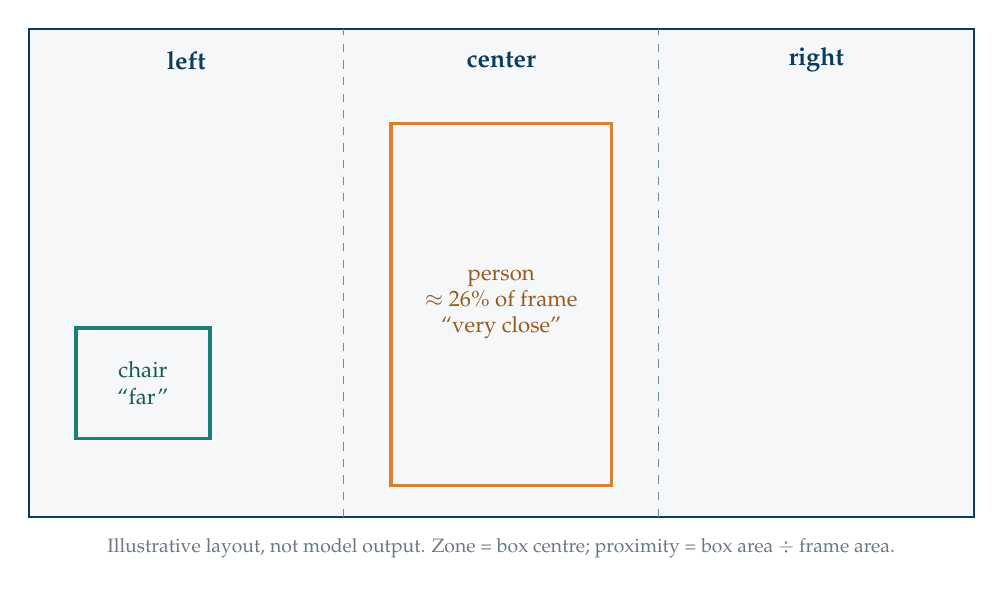
\begin{tikzpicture}[x=1cm,y=1cm]
  \draw[ink,thick,fill=paper] (0,0) rectangle (12,6.2);
  \draw[dashed,ink!60] (4,0) -- (4,6.2);
  \draw[dashed,ink!60] (8,0) -- (8,6.2);
  \node[ink,font=\small\bfseries] at (2,5.8) {left};
  \node[ink,font=\small\bfseries] at (6,5.8) {center};
  \node[ink,font=\small\bfseries] at (10,5.8) {right};
  \draw[saffron,very thick] (4.6,0.4) rectangle (7.4,5.0);
  \node[saffron!70!black,font=\footnotesize,align=center] at (6,2.7) {person\\ $\approx$ 26\% of frame\\ ``very close''};
  \draw[teal,very thick] (0.6,1.0) rectangle (2.3,2.4);
  \node[teal!70!black,font=\footnotesize,align=center] at (1.45,1.7) {chair\\ ``far''};
  \node[codegray,font=\scriptsize] at (6,-0.4) {Illustrative layout, not model output. Zone = box centre; proximity = box area $\div$ frame area.};
\end{tikzpicture}
\caption{Guidance logic: thirds of the frame give the side; the fraction of the frame covered by the box gives a coarse proximity class.}
\end{figure}

\subsection{The rules}
\begin{itemize}
  \item \textbf{Zone.} Let $c_x=(x_1+x_2)/(2W)$. Left if $c_x<1/3$, right if $c_x>2/3$, otherwise centre.
  \item \textbf{Proximity.} Let $r=\dfrac{(x_2-x_1)(y_2-y_1)}{WH}$. ``Very close'' if $r\ge0.30$, ``close'' if $r\ge0.08$, otherwise ``far''.
  \item \textbf{Ranking.} Sort by proximity, then hazard classes (person, vehicles, bicycle, dog, \dots), then centre before sides, then confidence. Speak at most three items.
  \item \textbf{No false reassurance.} With no detections the sentence is ``No known objects detected. This does not mean the way is clear.''
\end{itemize}
\begin{warnbox}[Monocular distance is crude]
Box area is a poor distance estimate: a bus far away and a chair nearby can cover the same fraction of the frame. The thresholds above are placeholders for a demonstration. For real use, calibrate against tape-measured distances per class (Chapter~\ref{ch:eval}), restrict claims to the classes you calibrated, or add a depth sensor (stereo camera, ToF, or ultrasonic).
\end{warnbox}

\lstinputlisting[style=py,caption={\texttt{netra/spatial.py}},label=lst:spatial]{../netra/spatial.py}
The \code{GuidanceThrottle} class prevents the system from repeating the same sentence every frame. It speaks when the message \emph{changes} (after a minimum gap) or when a repeat interval has passed, and takes an injectable clock so the unit test needs no real waiting.

\section{Object detection with a small YOLO model}
Install the optional dependency (this pulls in PyTorch and is a large download):
\begin{lstlisting}[style=sh]
pip install -r requirements-detect.txt
\end{lstlisting}
The code loads \code{models/yolo11n.pt} if it exists; otherwise it asks Ultralytics for \code{yolo11n.pt}, which is downloaded into the current directory on first use (move it into \code{models/} afterwards). Verify the current model names and download behaviour in the Ultralytics documentation; they change between releases. ``Nano'' models trade accuracy for speed, which suits edge devices.

\begin{warnbox}[Licensing]
Ultralytics software and weights are offered under the AGPL-3.0 licence or a separate commercial licence. The AGPL carries obligations for distribution and for network use. If you plan to distribute a product, read the current terms at the Ultralytics licence page and consider alternatives with permissive licences, or the commercial option.
\end{warnbox}

\lstinputlisting[style=py,caption={\texttt{netra/detection.py}},label=lst:detection]{../netra/detection.py}

\paragraph{Reading the code.}
\begin{itemize}
  \item \code{_get_model} loads the model lazily, so importing the agent does not require PyTorch.
  \item \code{detect_frame} works on an in-memory frame, which is what a live camera loop needs; \code{detect_objects} wraps it for files and writes an annotated copy.
  \item \code{guide_video} samples a video, builds guidance per sample, records only \emph{changes} in the sentence, and saves a JSON timeline. It also records per-frame latency, which feeds the evaluation in Chapter~\ref{ch:eval}.
  \item \code{benchmark_detector} performs a warm-up run before timing, because the first inference includes model loading and allocation.
  \item A confidence score is a model score, not a probability that the detection is correct.
\end{itemize}

\paragraph{Tracking (extension).} Detection answers ``what is in this frame''; tracking asks ``which detection corresponds to an object seen earlier''. Ultralytics provides \code{model.track(source=..., tracker="bytetrack.yaml")}. Tracking lets you say ``approaching'' by watching a box grow across frames, but identities can switch or vanish under occlusion, so treat them as estimates.

\section{Reading printed text}
OCR converts text in an image to characters. The tool upsamples small images, smooths slightly, binarises with Otsu's method, then calls Tesseract, which returns per-word confidences. Language codes follow Tesseract's three-letter convention (\code{eng}, \code{tel}, \code{hin}) and can be combined with \code{+}. Install language packs with \code{apt}, as in Chapter~3.
\lstinputlisting[style=py,caption={\texttt{netra/ocr\_tools.py}},label=lst:ocr]{../netra/ocr_tools.py}
Mean confidence is not accuracy. For safety-critical text such as medicine dosage, the system should tell the user that reading is uncertain and suggest human verification.

\section{Speech output}
\lstinputlisting[style=py,caption={\texttt{netra/speech.py}},label=lst:speech]{../netra/speech.py}
The text is passed on \emph{standard input} (\code{--stdin}) rather than as a command-line argument, so text beginning with a dash cannot be misread as an option, and the command is built as a list so no shell is involved. The file name is a hash of the voice, rate and text, so repeated phrases reuse the same WAV. Voices such as \code{te} (Telugu) and \code{hi} (Hindi) exist in espeak-ng; judge their intelligibility with real users before relying on them. Neural voices such as Piper may sound more natural; they are also open source but add model downloads.

\section{Scene description with a vision-language model}
A text-only LLM cannot see pixels. A vision-language model (VLM) accepts an image plus a question. Download one with \code{ollama pull llama3.2-vision} (large; check memory needs) and choose another with \code{NETRA_VISION}.
\lstinputlisting[style=py,caption={\texttt{netra/vision\_tools.py}},label=lst:vlm]{../netra/vision_tools.py}
The prompt tells the model to say ``unclear'' rather than guess and never to say a path is safe. A VLM \emph{describes}; it does not \emph{measure}. If the user needs exact positions, use detection; if they need exact text, use OCR.

\section{A deterministic pipeline}
Figure~\ref{fig:pipeline} shows \code{navigation_assist}. Because the steps are fixed, it is reproducible and does not depend on the LLM choosing correctly, which is how you would deploy the safety-relevant path on a device.
\begin{figure}[ht]
\centering
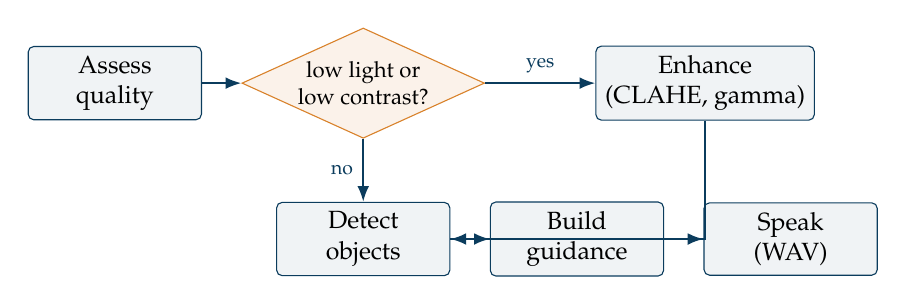
\begin{tikzpicture}[node distance=5mm,
  st/.style={draw=ink,rounded corners=2pt,fill=ink!6,font=\small,align=center,minimum height=9mm,minimum width=2.2cm},
  dec/.style={draw=saffron,diamond,aspect=2.2,fill=saffron!10,font=\footnotesize,align=center,inner sep=1pt},
  arr/.style={-{Latex[length=2mm]},thick,ink}]
\node[st] (a) {Assess\\ quality};
\node[dec,right=of a] (d) {low light or\\ low contrast?};
\node[st,right=14mm of d] (e) {Enhance\\ (CLAHE, gamma)};
\node[st,below=8mm of d] (f) {Detect\\ objects};
\node[st,right=of f] (g) {Build\\ guidance};
\node[st,right=of g] (h) {Speak\\ (WAV)};
\draw[arr] (a)--(d);
\draw[arr] (d)--node[above,font=\scriptsize]{yes}(e);
\draw[arr] (e)|-(f);
\draw[arr] (d)--node[left,font=\scriptsize]{no}(f);
\draw[arr] (f)--(g); \draw[arr] (g)--(h);
\end{tikzpicture}
\caption{The \code{navigation_assist} pipeline.}
\label{fig:pipeline}
\end{figure}
\lstinputlisting[style=py,caption={\texttt{netra/pipeline.py}},label=lst:pipeline]{../netra/pipeline.py}

% =====================================================================
\chapter{Connecting the Tools to the AI Agent}
% =====================================================================
\section{Function calling}
The model receives the user request, a system instruction and the \emph{schemas} of approved functions. For ``Enhance \code{hallway.png} with moderate brightening'' it may return a tool call such as \code{enhance_low_light(filename="hallway.png", gamma=1.8)}. \textbf{The Python program, not the model, executes it}, then returns the result so the model can explain what happened.

\section{The agent controller}
\lstinputlisting[style=py,caption={\texttt{netra/agent.py}},label=lst:agent]{../netra/agent.py}

\paragraph{How it works.}
\begin{enumerate}
  \item \code{TOOLS} is the allow-list. \code{TOOL_MAP} looks tools up by name. An unknown name is rejected and reported; the model cannot invoke anything else.
  \item \code{execute_tool} \emph{never raises}. Exceptions become \texttt{\{"error": \ldots\}} so the model can read what went wrong and correct its arguments.
  \item \code{_verify} checks that a file a tool claims to have written actually exists, implementing the rule ``verify the output, do not trust the explanation''.
  \item \code{run_query} is a \emph{bounded} loop: at most \code{MAX_ROUNDS} model calls per request, so a confused model cannot loop forever. Several tool calls in one reply are handled in order. This supports multi-step requests such as ``enhance, then detect''.
  \item Every call is appended to \code{output/reports/agent_log.jsonl} with time, tool, arguments, status and model name.
  \item The system prompt forbids claiming unperformed actions, inventing filenames or measurements, and declaring an area safe.
\end{enumerate}
\begin{notebox}[Client-version caveat]
The exact message format for tool results can change between Ollama client versions (for example, whether tool messages carry a call identifier). The code was checked only to the extent that all 22 functions convert into valid tool schemas with the \code{ollama} Python package. Test the full loop against your installed version and the official tool-calling documentation.
\end{notebox}

\section{Run the agent}
\begin{lstlisting}[style=sh]
cd ~/netra-ai
source .venv/bin/activate
python -m netra.agent
\end{lstlisting}
\code{-m} runs a module using package-aware imports, which is why you start from the project root. Example session (wording will vary by model):
\begin{lstlisting}[style=plain]
You: Is hallway.png too dark? Enhance it if so.
NetraAI: I assessed hallway.png (mean intensity 54, flagged low_light) and
ran enhance_low_light with clip_limit 2.0, tile_grid 8, gamma 1.8. The result
is saved at output/images/enhanced_hallway.png.
\end{lstlisting}
Always open the output file; do not rely only on the model's description of it.

\section{Hardening checklist}
\begin{itemize}
  \item Strict validation of every argument inside each tool (done) and image-size and video-length limits (done).
  \item Per-tool timeouts and cancellation for long videos (not yet implemented).
  \item Unique output names or run identifiers so repeated runs do not overwrite each other.
  \item Confirmation before overwriting or deleting anything.
  \item Never use \code{eval}, \code{exec} or a shell on model-generated text.
\end{itemize}

% =====================================================================
\chapter{Practical Experiments}
\label{ch:experiments}
% =====================================================================
Copy your own test images into \code{input/images/} and videos into \code{input/videos/}. Use your own recordings or images whose licence permits use. Do not use photographs of identifiable people without their consent. Each experiment lists the instruction, the tool the agent should choose, and what to verify. If the model chooses differently, that is a finding worth recording.

\begin{table}[ht]\centering\small
\begin{tabular}{@{}p{0.4cm}p{5.3cm}p{3.7cm}p{5.2cm}@{}}\toprule
\textbf{\#} & \textbf{Instruction} & \textbf{Expected tool} & \textbf{Verify}\\\midrule
1 & ``Give me the properties of \code{scene.png}.'' & \code{image_info} & Width, height, channels, size match \code{file}.\\
2 & ``Is \code{hallway.png} too dark? Fix it if needed.'' & \code{assess_image_quality}, then \code{enhance_low_light} & Reported mean intensity rises; parameters are reported.\\
3 & ``Remove salt-and-pepper noise from \code{noisy.png}.'' & \code{denoise_image} (median) & Isolated specks gone; edges intact. Ask the agent to compare median, Gaussian and bilateral if noise type is unknown.\\
4 & ``Read the text on \code{label.png} in English and Telugu.'' & \code{read_text} (\code{eng+tel}) & Compare against the true text; note the confidence.\\
5 & ``Extract one frame every 2 seconds from \code{walk.mp4}.'' & \code{extract_frames} & Count of saved frames $\approx$ duration$/2$.\\
6 & ``Detect objects in \code{street.png}.'' & \code{detect_objects} & Boxes drawn; zone and proximity sensible; sentence spoken.\\
7 & ``Analyse \code{walk.mp4} every 0.5 s.'' & \code{guide_video} & JSON timeline; mean latency reported.\\
8 & ``Run the full navigation pipeline on \code{corridor.png}.'' & \code{navigation_assist} & Steps list shows enhancement only if needed; WAV exists.\\
\bottomrule\end{tabular}
\caption{Agent experiments.}
\end{table}

\section{Controlled low-light experiment (measured)}
Real low-light footage has no clean reference, so image-quality metrics such as PSNR and SSIM cannot be computed. The standard remedy is a \emph{controlled} experiment: take a clean image, degrade it in a known way, enhance it, and compare with the original. The script \code{scripts/run_lowlight_experiment.py} does this with the astronaut photograph bundled with scikit-image, so it runs offline without extra downloads.
\begin{lstlisting}[style=sh]
python scripts/run_lowlight_experiment.py
\end{lstlisting}
The degradation is $I_{\text{dark}}=255\,(I/255)^{2.5}+\mathcal N(0,6^2)$ with a fixed random seed. Three enhancement settings are applied to the dark image.

\begin{figure}[ht]
\centering
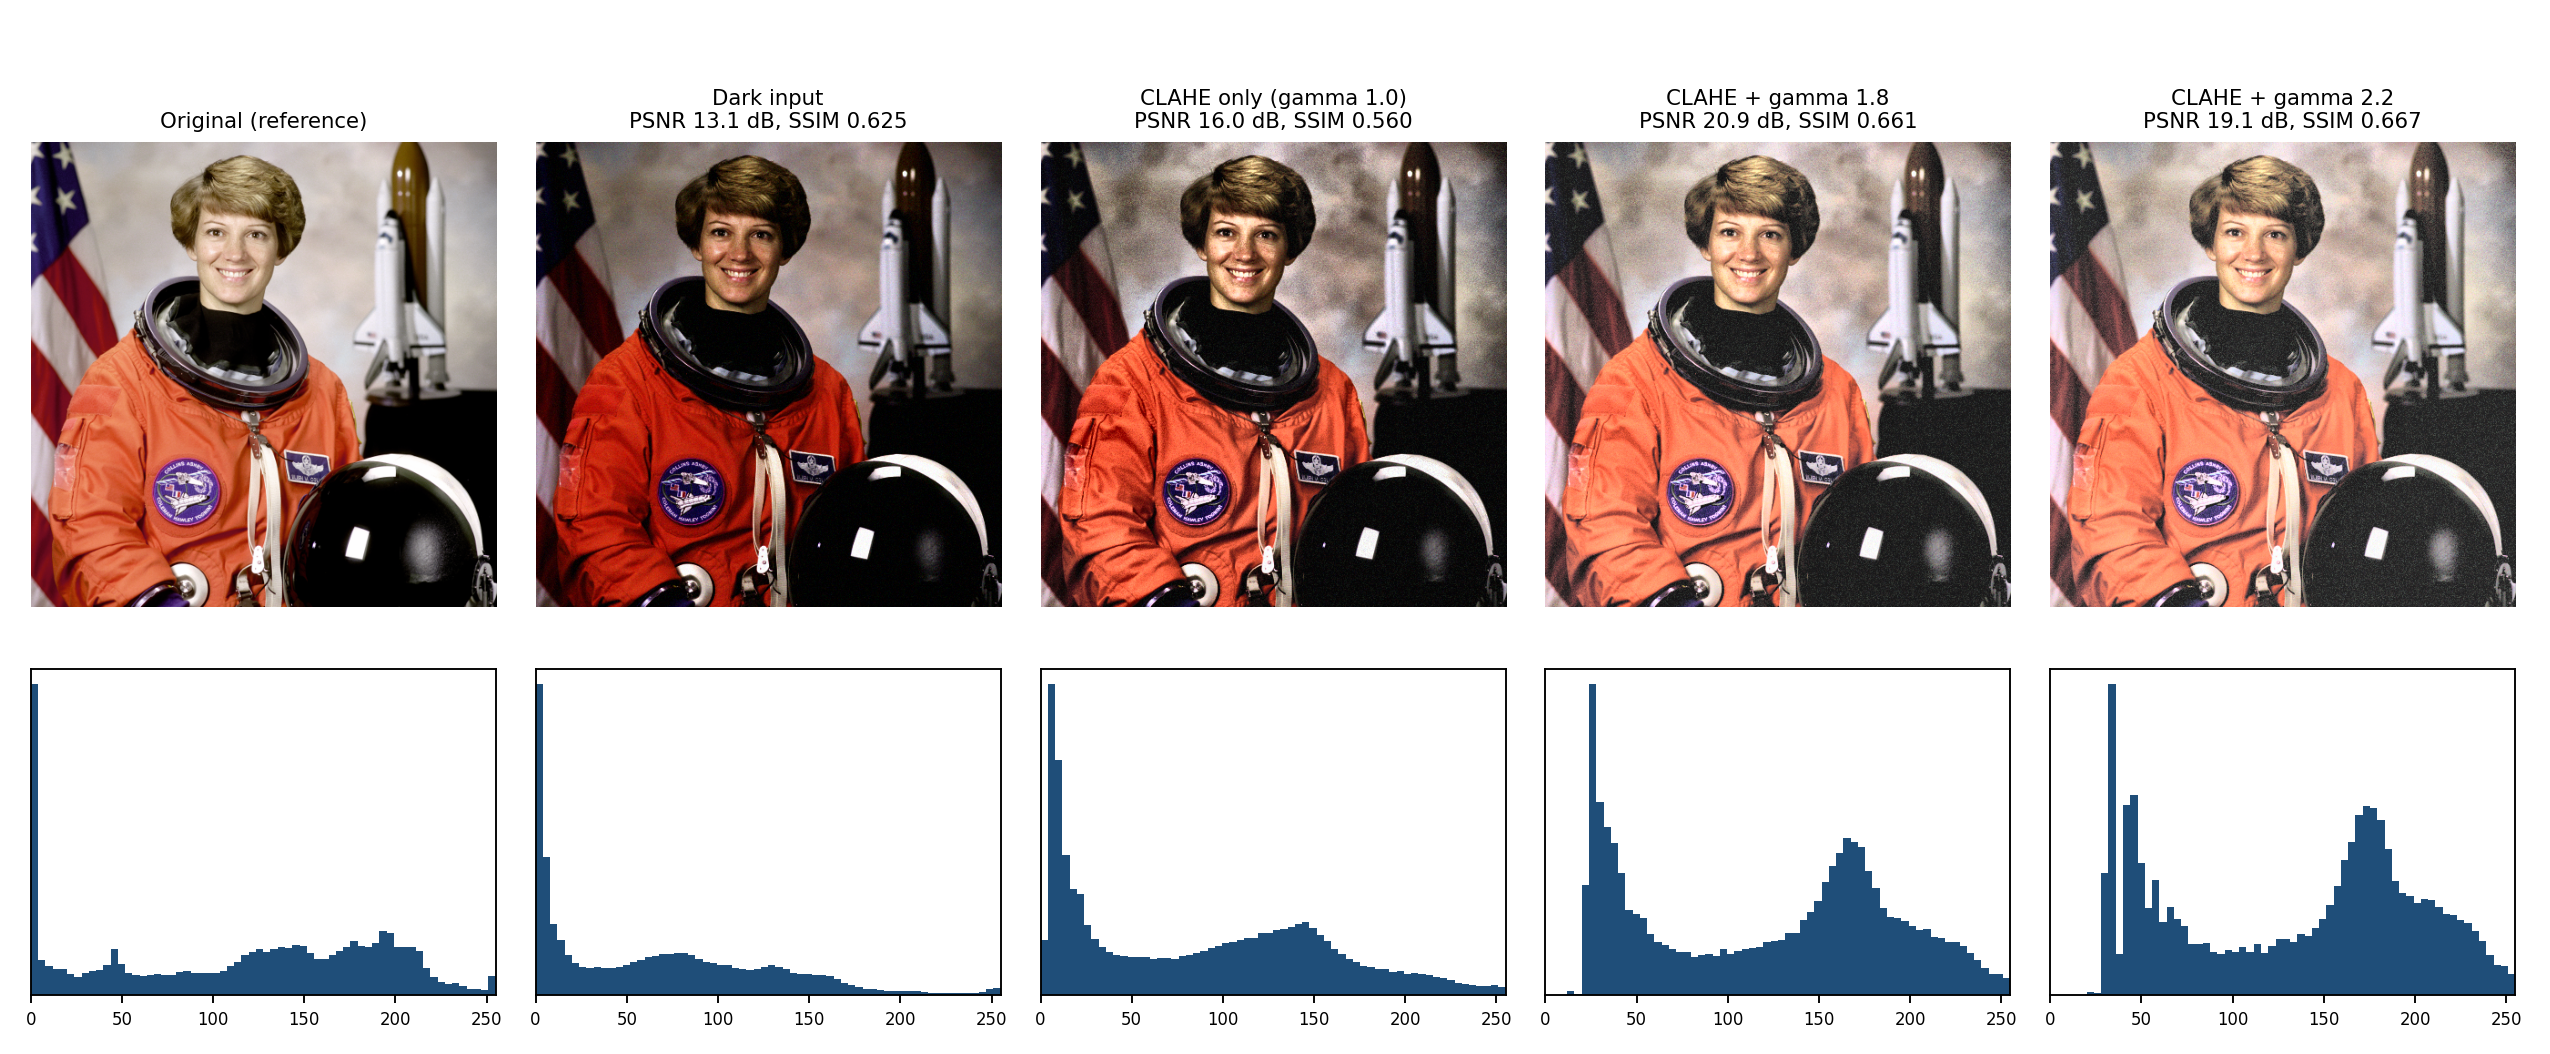
\includegraphics[width=\textwidth]{figures/lowlight_experiment.png}
\caption{Top: original, degraded input, and three enhancements. Bottom: grayscale histograms. PSNR and SSIM are computed against the original on the grayscale versions.}
\label{fig:lowlight}
\end{figure}

\begin{table}[ht]\centering\small
\begin{tabular}{@{}lrrr@{}}\toprule
\textbf{Image} & \textbf{PSNR (dB)} & \textbf{SSIM} & \textbf{Mean intensity}\\\midrule
Dark input & 13.05 & 0.625 & 65.7\\
CLAHE only ($\gamma=1.0$) & 16.04 & 0.560 & 86.7\\
CLAHE + gamma 1.8 & 20.88 & 0.661 & 121.7\\
CLAHE + gamma 2.2 & 19.11 & 0.668 & 133.6\\
\bottomrule\end{tabular}
\caption{Measured results (one image, one seed). Clip limit 2.0 and an $8\times8$ tile grid throughout.}
\end{table}

\paragraph{What the numbers do and do not say.}
\begin{itemize}
  \item CLAHE alone \emph{raised} PSNR but \emph{lowered} SSIM below the dark input. A likely explanation is that local contrast stretching also amplifies the added noise, which SSIM's structure term penalises; the evidence here (a single image) is suggestive, not conclusive. This is a good illustration of why one metric is never enough.
  \item Adding gamma 1.8 gave the highest PSNR; gamma 2.2 gave the highest SSIM but lower PSNR. There is no single ``best'' setting; it depends on the criterion, and the criterion should match the task (for example detection accuracy downstream).
  \item The result is for one synthetic degradation of one image. Do not generalise. Repeat over many images, several degradations and multiple seeds, and report mean and spread.
  \item PSNR and SSIM measure similarity to the original, not usefulness to a blind user or to a detector. The real test of an enhancement step is whether detection recall improves on genuinely dark frames (Chapter~\ref{ch:eval}).
\end{itemize}

% =====================================================================
\chapter{Evaluation}
\label{ch:eval}
% =====================================================================
\section{Image-quality metrics}
For a reference $I$ and a processed image $K$ of size $M\times N$:
\[
\text{MSE}=\frac{1}{MN}\sum_{x,y}\big[I(x,y)-K(x,y)\big]^2,\qquad
\text{PSNR}=10\log_{10}\frac{\text{MAX}_I^2}{\text{MSE}},
\]
with $\text{MAX}_I=255$ for 8-bit images (PSNR is infinite if the images are identical). SSIM compares luminance, contrast and structure in local windows:
\[
\text{SSIM}(x,y)=\frac{(2\mu_x\mu_y+C_1)(2\sigma_{xy}+C_2)}{(\mu_x^2+\mu_y^2+C_1)(\sigma_x^2+\sigma_y^2+C_2)}.
\]

\section{Detection metrics}
Match each prediction to a ground-truth box of the same class when their intersection over union exceeds a threshold (commonly $0.5$):
\[
\text{IoU}(A,B)=\frac{|A\cap B|}{|A\cup B|},\quad
P=\frac{TP}{TP+FP},\quad R=\frac{TP}{TP+FN},\quad F_1=\frac{2PR}{P+R}.
\]
For an assistive device \emph{recall on hazard classes} and \emph{false alarms per minute} usually matter more than overall accuracy. Report them separately for each lighting condition, because average performance hides failures in the dark.

\lstinputlisting[style=py,caption={\texttt{netra/metrics.py}},label=lst:metrics]{../netra/metrics.py}
\code{compare_images} takes the reference from \code{input/} and the processed image from \code{output/} (or \code{input/}); \code{simulate_low_light} creates the controlled degradation; \code{iou} and \code{precision_recall} are pure functions with unit tests. Greedy matching in descending confidence order is a simplification of the full mAP protocol; use the evaluation tools in your detection framework for published numbers.

\section{Task-level and system-level measures}
\begin{table}[ht]\centering\small
\begin{tabular}{@{}p{3.7cm}p{6cm}p{5cm}@{}}\toprule
\textbf{Measure} & \textbf{How to obtain it} & \textbf{Why it matters}\\\midrule
Hazard recall, precision & Annotate 200+ frames per condition; run \code{precision_recall} & Missed hazards and false alarms.\\
Zone accuracy & Compare predicted left/center/right with annotated side & Wrong side is worse than no message.\\
Proximity calibration & Place objects at measured distances; tabulate predicted class vs. true distance per class & Validates or replaces the area heuristic.\\
End-to-end latency & Time capture $\rightarrow$ detection $\rightarrow$ sentence $\rightarrow$ audio start & Stale guidance is misleading.\\
Throughput (FPS) & \code{benchmark_detector} on the target device & Feasibility on edge hardware.\\
False alarms per minute & Run on hazard-free footage & Alert fatigue.\\
Speech intelligibility & Listening tests with target users and languages & Usability.\\
Enhancement value & Detection recall with vs.\ without enhancement on real dark frames & The real test of Chapter~5 enhancement.\\
\bottomrule\end{tabular}
\caption{Evaluation plan for an assistive-vision prototype.}
\end{table}

\begin{table}[ht]\centering\small
\begin{tabular}{@{}lp{9cm}@{}}\toprule
\textbf{Stage} & \textbf{Latency budget (design target to verify, not a measurement)}\\\midrule
Capture and decode & as short as the camera allows\\
Quality check and enhancement & small compared with inference\\
Detection & dominant cost; depends on model, input size, device\\
Guidance sentence & negligible\\
Speech synthesis start & short for espeak-ng; longer for neural voices\\
\bottomrule\end{tabular}
\end{table}
Measure each stage separately on the target device, set an end-to-end target with your mobility instructors (how stale can a message be before it misleads?), and report percentiles, not only the mean.

\section{Testing and reproducibility}
The test suite checks path rejection, invalid arguments, quality flags, an enhancement improving PSNR on a darkened synthetic image, video sampling and motion detection on a generated clip, spatial rules, the throttle, IoU and precision/recall, and detection post-processing with a stand-in model. Excerpt:
\lstinputlisting[style=py,firstline=1,lastline=40,caption={\texttt{tests/test\_spatial.py}},label=lst:testspatial]{../tests/test_spatial.py}
For research reproducibility, record with each result: input file checksum (\code{sha256sum}), model name and version, library versions (\code{pip freeze}), all parameters (the tools return them), a timestamp, and the output checksum. The agent log already stores tool, arguments, status and model.

% =====================================================================
\chapter{Interfaces: Streamlit and the Live Loop}
% =====================================================================
\section{Streamlit}
\begin{lstlisting}[style=sh]
streamlit run app.py
\end{lstlisting}
Streamlit turns the Python script into a local web app, usually at \code{http://localhost:8501}. Under WSL, open that address in the Windows browser.
\lstinputlisting[style=py,caption={\texttt{app.py}},label=lst:app]{../app.py}
Two tabs are provided: direct tool buttons (assess, enhance, detect and speak) and a chat tab that calls the agent and keeps a short history. For a deployed app, use unique server-generated filenames (the example derives one), enforce upload size limits, authenticate users, and do not trust uploaded filenames.

\section{Live guidance from a camera or a video file}
\begin{lstlisting}[style=sh]
python -m netra.live --source street.mp4 --max-seconds 30
python -m netra.live --source 0              # first webcam (native Ubuntu / Pi)
\end{lstlisting}
\lstinputlisting[style=py,caption={\texttt{netra/live.py}},label=lst:live]{../netra/live.py}
The loop analyses a frame every \code{--step} seconds, builds the guidance sentence, and lets \code{GuidanceThrottle} decide whether to speak. Speech runs in a separate process so it never blocks capture, and a new utterance is not started while the previous one is still playing. Recorded video files make the loop testable in WSL and repeatable for evaluation.

% =====================================================================
\chapter{Edge Deployment}
% =====================================================================
A wearable needs the detection and guidance path to run on a small board. The LLM agent is a development and research tool; on the device you would normally run only the deterministic pipeline.

\section{Design levers}
\begin{itemize}
  \item \textbf{Input size.} Inference cost grows roughly with pixel count. Try \code{imgsz=320} before 640 and measure recall loss.
  \item \textbf{Frame skipping.} Analyse two frames per second, not thirty; walking speed does not need more for coarse guidance.
  \item \textbf{Model format.} Export the model to a lighter runtime (ONNX, NCNN, TFLite) and benchmark each on the device.
  \item \textbf{Throttle speech.} Avoid repetition (\code{GuidanceThrottle}); fewer, better messages beat constant chatter.
  \item \textbf{Thermals and power.} Sustained inference throttles small boards; measure over minutes, not seconds, and measure battery life.
  \item \textbf{Audio path.} Bone-conduction or open-ear Bluetooth headphones keep ambient sound audible; account for Bluetooth latency.
\end{itemize}

\section{Exporting a model}
\begin{lstlisting}[style=py]
from ultralytics import YOLO
model = YOLO("yolo11n.pt")
model.export(format="onnx", imgsz=320)      # also e.g. format="ncnn" or "tflite"
\end{lstlisting}
Supported formats and their runtime requirements change; consult the Ultralytics export documentation for your version. Verify that detection quality after export matches the original on your own validation set.

\section{On the Raspberry Pi}
\begin{enumerate}
  \item Install Raspberry Pi OS or Ubuntu, then repeat the apt and virtual-environment steps of Chapter~3 (skip Ollama; it is too heavy for the smallest boards).
  \item Run \code{python -m pytest -q} to check the core pipeline on ARM.
  \item Run \code{python -m netra.live --source 0 --step 0.5} and note the printed latency per analysed frame.
  \item Record latency distribution, memory use, temperature and battery drain over a 30-minute run.
\end{enumerate}
Small boards such as the Zero 2~W have very limited memory and CPU. If your measured latency does not meet your target, options are a faster board, a smaller input size, a lighter export format, or an accelerator. Decide from measurements, not assumptions.

% =====================================================================
\chapter{Reliability, Safety, Privacy and Ethics}
% =====================================================================
\section{Failure modes and safeguards}
\begin{table}[ht]\centering\small
\begin{tabular}{@{}p{4.1cm}p{10.6cm}@{}}\toprule
\textbf{Problem} & \textbf{Safeguard}\\\midrule
Missed hazard & Report recall per class and condition; never claim the way is clear; keep traditional aids.\\
False alarms & Confidence threshold, throttle, per-class tuning; measure alarms per minute.\\
Wrong side or distance & Calibrate zones and proximity; restrict claims to calibrated classes.\\
Motion blur, glare, darkness & Quality assessment, enhancement, and a spoken ``image unclear'' message when quality is too low.\\
Wrong tool or parameters & Allow-list, in-tool validation, bounded rounds, logged calls.\\
Model invents results & Rule ``never claim without a tool result''; verify output files exist.\\
Path traversal or arbitrary execution & Plain filenames only; no shell, \code{eval} or \code{exec} on model text.\\
Resource exhaustion & Image-size and video-length limits; add timeouts and concurrency limits.\\
Overwriting data & Prefix outputs; keep originals read-only in practice.\\
Misreading text & Report OCR confidence; recommend human verification for medicine or safety text.\\
\bottomrule\end{tabular}
\end{table}

\section{Operational rules}
\begin{enumerate}
  \item Keep the Ollama API bound to a trusted local interface unless a secure network design is deliberate.
  \item Restrict file access to the project directories.
  \item Record the selected algorithm and all parameters; preserve originals.
  \item Ask for confirmation before destructive or expensive operations.
  \item Set a maximum number of tool-call rounds (done) and log errors.
\end{enumerate}

\section{Privacy}
A wearable camera captures bystanders. Process locally, do not store frames longer than needed, avoid uploading, and tell people nearby when recording. Do not commit personal images or video to GitHub (the \code{.gitignore} excludes \code{input/} and \code{output/}). Check local law on recording in public and private spaces.

\section{Working with users}
Involve visually impaired users and orientation-and-mobility professionals from the start, not only at the end. Ask what information they want, how often, and in which language and voice. An evaluation with participants needs institutional ethical approval and informed consent. Avoid describing the system as improving ``safety'' until you have evidence.

% =====================================================================
\chapter{Publishing the Project on GitHub}
% =====================================================================
\section{Before the first commit}
\begin{itemize}
  \item Replace the name placeholder in \code{LICENSE} and the repository URL in \code{README.md} and in \code{docs/netra_tutorial.tex}.
  \item Confirm \code{.gitignore} excludes \code{.venv/}, \code{input/}, \code{output/}, model weights and LaTeX build files.
  \item Make sure no secrets, personal photographs or recordings are in the tree.
  \item Decide the licence. MIT is permissive for your own code, but dependencies keep their own licences; in particular read the Ultralytics terms before distributing anything that depends on it.
\end{itemize}

\section{Create the local repository}
\begin{lstlisting}[style=sh]
git config --global user.name "Your Name"
git config --global user.email "you@example.com"
cd ~/netra-ai
git init -b main
git add .
git status
git commit -m "Initial commit: NetraAI assistive-vision agent"
\end{lstlisting}
\code{git init -b main} creates a repository whose first branch is \code{main}. \code{git add .} stages everything not ignored. \textbf{Read the output of \code{git status}}: if \code{input/}, \code{output/} or any \code{.pt} file appears, fix \code{.gitignore} before committing. \code{git commit -m} records the snapshot with a message.

\section{Create the GitHub repository}
On github.com choose \emph{New repository}, name it (for example \code{netra-ai}), and create it \emph{empty}: no README, licence or \code{.gitignore}, because you already have them locally.

\section{Authenticate}
An SSH key is convenient for WSL.
\begin{lstlisting}[style=sh]
ssh-keygen -t ed25519 -C "you@example.com"
cat ~/.ssh/id_ed25519.pub
\end{lstlisting}
Copy the printed public key into GitHub under \emph{Settings $\rightarrow$ SSH and GPG keys $\rightarrow$ New SSH key}, then test:
\begin{lstlisting}[style=sh]
ssh -T git@github.com
\end{lstlisting}
Never share the private key (\code{id_ed25519} without \code{.pub}). Alternatively use HTTPS with a personal access token or the GitHub CLI.

\section{Push}
\begin{lstlisting}[style=sh]
git remote add origin git@github.com:<your-user>/netra-ai.git
git push -u origin main
\end{lstlisting}
\code{remote add} names the remote \code{origin}; \code{push -u} uploads \code{main} and remembers the upstream so later you can simply run \code{git push}. After the push, the workflow in \code{.github/workflows/ci.yml} runs the test suite on every push and pull request; check the \emph{Actions} tab for a green result.

\section{Good practice afterwards}
\begin{itemize}
  \item Work on branches (\code{git switch -c feature/ocr-confidence}) and merge through pull requests.
  \item Tag releases: \code{git tag -a v0.1.0 -m "First release"} then \code{git push origin v0.1.0}.
  \item Put the compiled tutorial PDF in \code{docs/} so readers can open it from the repository, and keep experiment outputs small. For larger sample media use Git LFS (\code{git lfs install}; \code{git lfs track "*.mp4"}) or link to a dataset host, and check the licence of any dataset you redistribute.
  \item Add a short ``Validation status'' section to the README listing what you tested on which hardware, as this project does.
  \item If you ever commit a secret by mistake, rotating the secret is required; deleting the file in a later commit does not remove it from history.
\end{itemize}

\section{Building this document}
\begin{lstlisting}[style=sh]
sudo apt install -y texlive-latex-extra texlive-fonts-recommended latexmk
cd docs
latexmk -pdf netra_tutorial.tex
\end{lstlisting}
The listings are included from the source files, so rebuilding the PDF after changing the code updates the document. Run \code{python scripts/run_lowlight_experiment.py} first if you want to regenerate the figure.

% =====================================================================
\chapter{Roadmap and Hardware}
% =====================================================================
\begin{table}[ht]\centering\small
\begin{tabular}{@{}clp{8cm}@{}}\toprule
\textbf{Phase} & \textbf{Activity} & \textbf{Deliverable}\\\midrule
1 & WSL2/Ubuntu environment, tests passing & Reproducible setup\\
2 & Image-quality tools and controlled experiments & Enhancement study with metrics\\
3 & Video tools, recorded walking footage (with consent) & Annotated evaluation set\\
4 & Detection, zones, proximity calibration & Per-class recall and calibration table\\
5 & OCR and speech in English, Telugu and Hindi & Intelligibility results with users\\
6 & Agent with Ollama, logging, bounded loop & Verified tool calling on your client version\\
7 & Edge export and Raspberry Pi benchmark & Latency, thermal and battery data\\
8 & User study with ethical approval & Findings and design changes\\
9 & Tracking, depth sensing, haptic output & V2 prototype\\
\bottomrule\end{tabular}
\end{table}

\begin{table}[ht]\centering\small
\begin{tabular}{@{}p{3.3cm}p{11.4cm}@{}}\toprule
\textbf{Component} & \textbf{Suggested configuration}\\\midrule
Development PC & Modern Intel Core i5/i7 or AMD Ryzen 5/7; 16 GB RAM minimum, 32 GB more comfortable for local models; about 100 GB free disk.\\
GPU (optional) & NVIDIA GPU with current driver; CPU is enough for this tutorial.\\
Camera & USB webcam or Raspberry Pi camera; fixed mounting for repeatable tests.\\
Edge board & Raspberry Pi-class board; choose by measured latency, not by price alone.\\
Audio & Open-ear or bone-conduction headphones.\\
Network & Internet for initial downloads; local processing afterwards.\\
\bottomrule\end{tabular}
\caption{Planning guidelines, not guaranteed minimums. Actual needs depend on model size, quantisation, resolution and concurrent jobs.}
\end{table}

% =====================================================================
\chapter{Official Documentation and Further Reading}
% =====================================================================
\begin{table}[ht]\centering\small
\begin{tabular}{@{}p{3.6cm}p{11cm}@{}}\toprule
\textbf{Software} & \textbf{Official resource}\\\midrule
Ollama & \url{https://docs.ollama.com/}\\
Ollama tool calling & \url{https://docs.ollama.com/capabilities/tool-calling}\\
Ollama Python client & \url{https://github.com/ollama/ollama-python}\\
OpenCV & \url{https://docs.opencv.org/}\\
scikit-image & \url{https://scikit-image.org/docs/stable/}\\
Ultralytics & \url{https://docs.ultralytics.com/} and \url{https://www.ultralytics.com/license}\\
Tesseract & \url{https://tesseract-ocr.github.io/}\\
espeak-ng & \url{https://github.com/espeak-ng/espeak-ng}\\
FFmpeg & \url{https://ffmpeg.org/documentation.html}\\
Streamlit & \url{https://docs.streamlit.io/}\\
WSL & \url{https://learn.microsoft.com/windows/wsl/}\\
GitHub docs & \url{https://docs.github.com/}\\
\bottomrule\end{tabular}
\end{table}

\chapter*{Conclusion}
\addcontentsline{toc}{chapter}{Conclusion}
NetraAI separates concerns: a language model interprets requests and chooses from approved tools; deterministic libraries do the processing; a small, testable guidance layer turns detections into short spoken sentences without claiming more than the evidence supports. Start with the parts you can verify today, namely quality assessment, enhancement, metrics and the test suite. Then add detection, speech and the agent loop one at a time, and measure each on your own data and hardware. Treat the system as a research tool, involve the people it is meant to serve, and report limitations as carefully as results.


\end{document}
